\begin{figure}[H]
\centering

% --- Left: Optimality gap ---
\begin{subfigure}{0.48\linewidth}
\centering
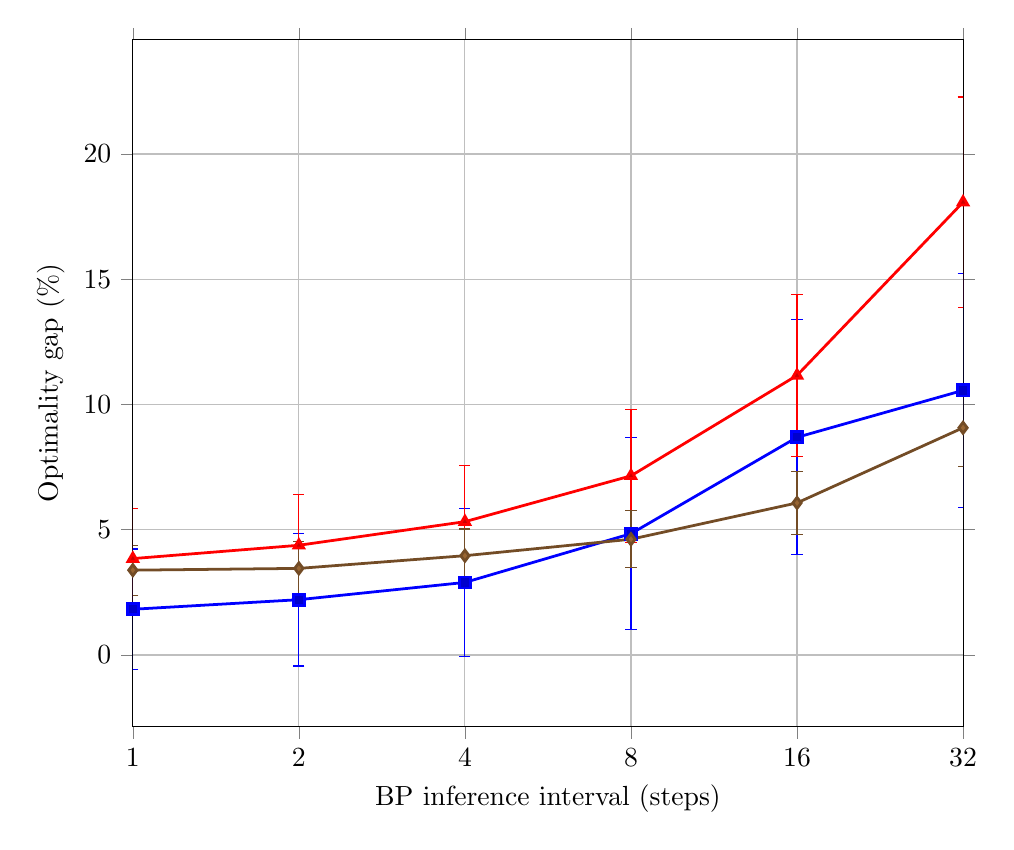
\begin{tikzpicture}
\begin{axis}[
  width=\linewidth, height=0.85\linewidth,
  xmode=log, log basis x={2},
  xmin=1, xmax=32,
  xtick={1,2,4,8,16,32},
  xticklabels={1,2,4,8,16,32},
  xlabel={BP inference interval (steps)},
  ylabel={Optimality gap (\%)},
  ymajorgrids, grid=both,
  tick align=outside,
  legend to name=sharedlegend,   % <-- share legend
  legend columns=2
]
  % MIS(n=100) (gap)
  \addplot+[
    mark=square*,
    line width=1pt,
    error bars/.cd, y dir=both, y explicit
  ] coordinates {
    (1, 1.824) +- (0, 2.405)
    (2, 2.207) +- (0, 2.646)
    (4, 2.896) +- (0, 2.957)
    (8, 4.842) +- (0, 3.830)
    (16, 8.688) +- (0, 4.694)
    (32, 10.563) +- (0, 4.664)
  };
  \addlegendentry{MIS ($n=100$)}

  % MIS(n=[200;300]) (gap)
  \addplot+[
    mark=triangle*,
    line width=1pt,
    error bars/.cd, y dir=both, y explicit
  ] coordinates {
    (1, 3.847) +- (0, 1.988)
    (2, 4.379) +- (0, 2.038)
    (4, 5.321) +- (0, 2.244)
    (8, 7.151) +- (0, 2.651)
    (16, 11.160) +- (0, 3.238)
    (32, 18.074) +- (0, 4.200)
  };
  \addlegendentry{MIS ($n\sim [200,300]$)}

  % Dataset B (gap)
  \addplot+[
    mark=diamond*,
    line width=1pt,
    error bars/.cd, y dir=both, y explicit
  ] coordinates {
    (1, 3.385  ) +- (0, 0.995 )
    (2, 3.456  ) +- (0, 1.058 )
    (4, 3.963  ) +- (0, 1.064 )
    (8, 4.62   ) +- (0, 1.131 )
    (16, 6.07   ) +- (0, 1.248 )
    (32, 9.07) +- (0, 1.56)
  };
  \addlegendentry{MIS ($n\sim [700,800]$)}
\end{axis}
\end{tikzpicture}
%\caption{Optimality gap}
\end{subfigure}
\hfill
% --- Right: Runtime ---
\begin{subfigure}{0.48\linewidth}
\centering
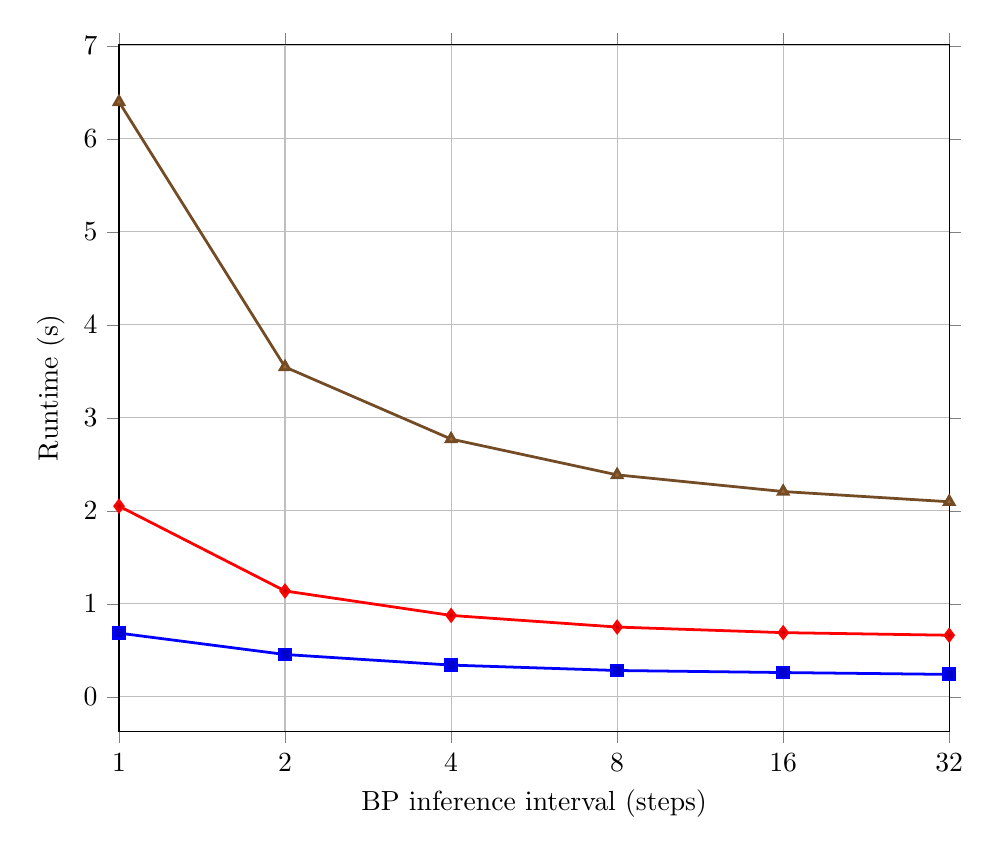
\begin{tikzpicture}
\begin{axis}[
  width=\linewidth, height=0.85\linewidth,
  xmode=log, log basis x={2},
  xmin=1, xmax=32,
  xtick={1,2,4,8,16,32},
  xticklabels={1,2,4,8,16,32},
  xlabel={BP inference interval (steps)},
  ylabel={Runtime (s)},
  ymajorgrids, grid=both,
  tick align=outside,
  %legend to name=sharedlegend,   % <-- same name
  legend columns=2
]
  % Dataset A (runtime)
  \addplot+[
    mark=square*,
    %dashed,
    line width=1pt
  ] coordinates {
    (1, 0.686) (2, 0.456) (4, 0.342)
    (8, 0.284) (16, 0.262) (32, 0.242)
  };
  %\addlegendentry{MIS ($n=100$)}

  % MIS (n=[200;300]) (runtime)
  \addplot+[
    mark=diamond*,
    %dashed,
    line width=1pt
  ] coordinates {
    (1, 2.051) (2, 1.139) (4, 0.876)
    (8, 0.751) (16, 0.691) (32, 0.663)
  };
  %\addlegendentry{MIS ($n\sim [200,300]$)}

  % MIS (n=[700;800]) (runtime)
  \addplot+[
    mark=triangle*,
    %dashed,
    line width=1pt
  ] coordinates {
    (1, 6.397) (2, 3.547) (4, 2.772)
    (8, 2.387) (16, 2.208) (32, 2.098)
  };
  %\addlegendentry{MIS ($n\sim [700,800]$)}
\end{axis}
\end{tikzpicture}
%\caption{Runtime}
\end{subfigure}

% --- Print shared legend once (after both axes are built)
\vspace{0.4em}
\pgfplotslegendfromname{sharedlegend}

\caption{Effect of BP inference frequency on (left) optimality gap and (right) runtime, with one shared legend. These values were obtained for the canonical probability model, the values of $\EPARAM$ were not learned.}
\label{fig:bp_gap_runtime_split}
\end{figure}